\documentclass{standalone}

\usepackage[dvipsnames]{xcolor}
\usepackage{tikz}

\begin{document}

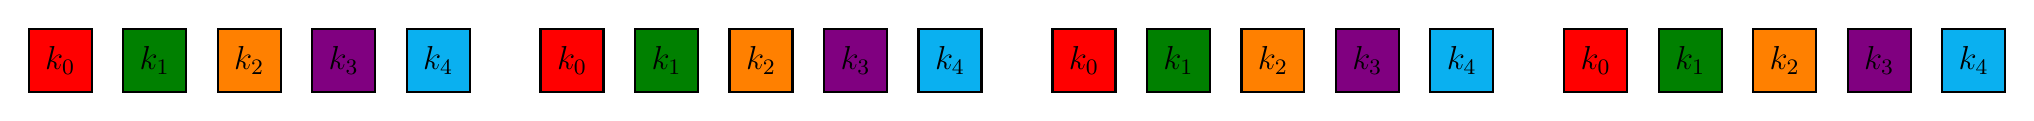
\begin{tikzpicture}[thick]
  \foreach \b in {0, ..., 3} {
    \foreach \i/\c in {0/Red, 1/Green, 2/orange, 3/Purple, 4/ProcessBlue} {
      \draw [fill=\c] ({(\b * 5) * 1.3cm + \i * 1.2cm }, 0)
            rectangle ++(0.8cm, 0.8cm) node [midway] {\large$k_\i$};
    }
  }
\end{tikzpicture}
\end{document}
